\subsection{Experimental Setup}
In this section, we empirically evaluate the effectiveness and interpretability of the proposed~\dname~on both
simulation and real-world datasets.
For interpretability, we focus on whether the algorithm can uncover the causal relationships inherent in the knowledge graph.


\subsubsection{\textbf{Baselines}}
% The aim of this experiment was to evaluate both the effectiveness and interpretability of the existing methods and our approach.
% In this paper, we design a causal rule-based prediction algorithm mainly for application scenarios that require explainability.
To evaluate the interpretability of the algorithms, we select four rule-based methods
that can conduct link prediction and generate explainable rules.
To make a fair comparison, the inference rules, obtained from different algorithms, are used to conduct the link prediction task based on the same prediction equations.
This approach can also help us observe the impact of different rules on the link prediction task.
For a complete evaluation of the effectiveness of the proposed approach, we also compute the LP performance of TuckER\cite{balazevic2019tucker}, one representation-based method which has the best overall performance among the representation-based methods across different datasets\cite{rossi2021knowledge}.
All baselines are listed in the following:
\begin{itemize}
\item[1)] AMIE+\cite{galarraga2015fast}, an efficient  top-down method to discover the interpretable rules.
\item[2)] AnyBURL\cite{meilicke2019anytime}, a bottom-up approach to mine the logical rule.
\item[3)] Neural-LP\cite{yang2017differentiable}, an end-to-end differentiable model to learn the first-order logical rule.
\item[4)] RNNLogic\cite{qu2020rnnlogic}, an EM-based algorithm to learn the rule generator and the reasoning predictor iteratively.
\item[5)] TuckER\cite{balazevic2019tucker},  a linear model based on Tucker
decomposition of the binary tensor representation of knowledge graph triples.
\end{itemize}





\subsubsection{\textbf{Datasets}}
To quantitatively evaluate the effectiveness of the algorithm in discovering causal knowledge, we construct a simulation dataset owing to a lack of groundtruth of real datasets.
Douban and Hetionet~\cite{himmelstein2017systematic} are selected as our real datasets on which we perform two link prediction tasks, movie rating prediction and drug repurposing, respectively.
Here we provide more details for these datasets, and their statistics are shown in Table~\ref{tab:dataset_statistics}.

% \begin{figure}[t]
% \vspace{0cm}
% \centering
% 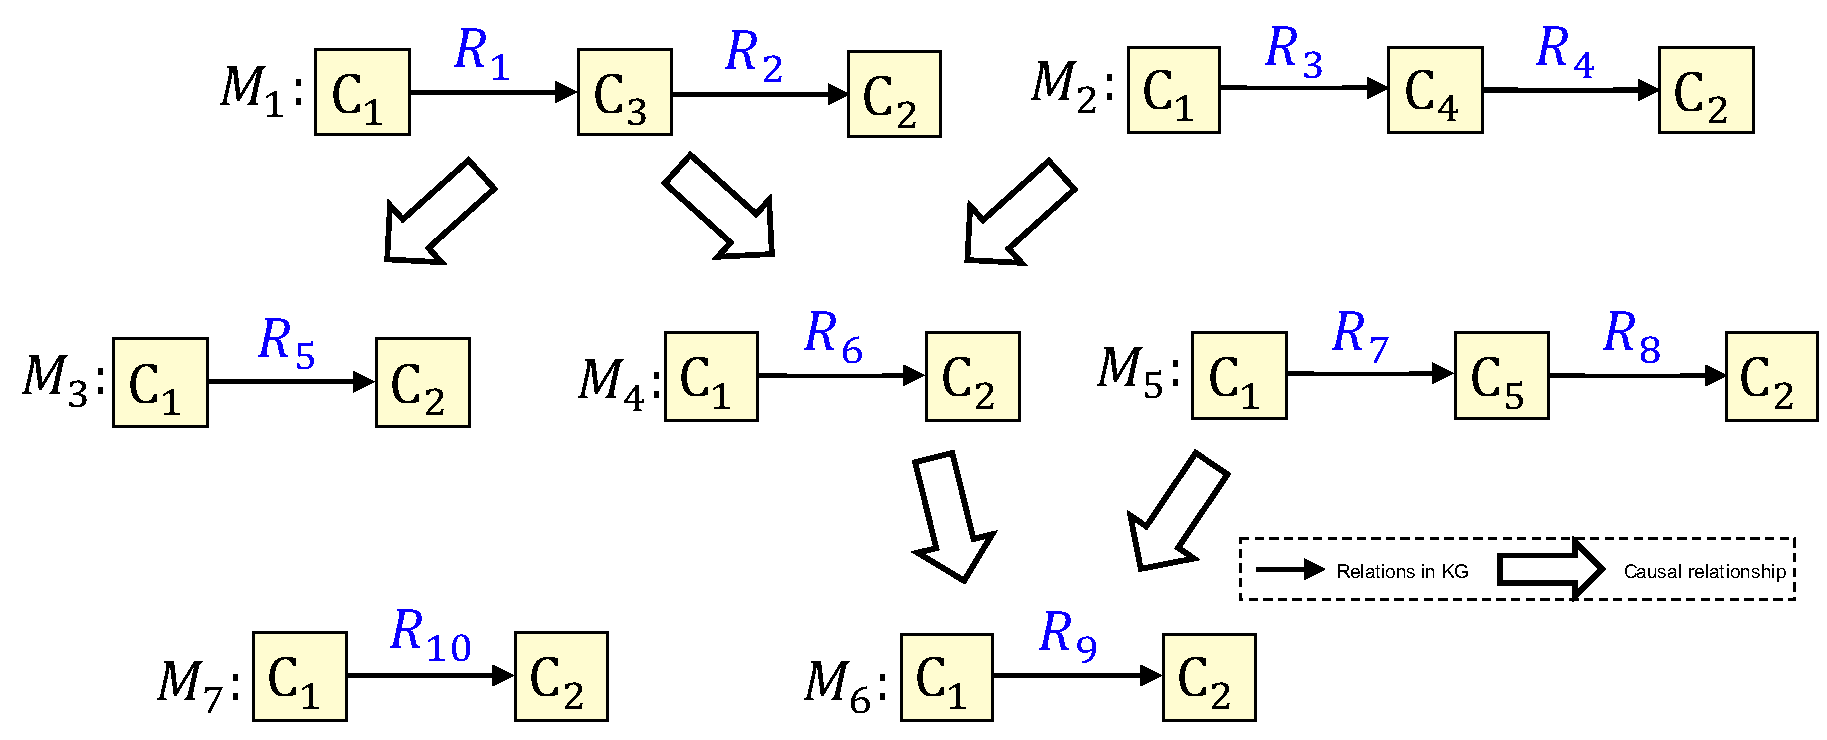
\includegraphics[width=8.5cm]{./figures/simulation.pdf}
% \caption{ The causal graph used to generate simulated knowledge graphs.}
% \label{fig:toy_example}
% \end{figure}

\begin{table}[t]
\centering
\caption{Dataset statistics of all the experiments.}
\label{tab:dataset_statistics}
% \vspace{-2pt}
\scalebox{1}{
\begin{tabular}{c|ccc}
\hline
   & \textbf{\#Triplets} & \textbf{\#Relations} & \textbf{\#Entities}  \\
\hline
\textbf{Simulation} & 6,095 & 5 & 1,590\\
\textbf{Douban Movie Rate} & 28,356 & 12 & 3,007 \\
\textbf{Hetionet} & 174,941 & 20 & 32,056 \\
\hline
\end{tabular}
}
\end{table}

\noindent
{\bf Simulation dataset.}
We generate simulated KGs based on a toy causal model specified in Fig.~\ref{fig:simulation}, which includes three concepts and five relations.
In particular, we design the causal mechanisms in KG via a probabilistic model.
The root nodes ($X_1$, $X_4$) in the causal graph are generated via Bernoulli distributions, whose probability mass function is $f_X(x)=p^x(1-p)^{1-x}$.
Moreover, the non-root nodes ($X_2$, $X_3$) are generated via the conditional probability distributions, which are Bernoulli distributions, given the parent node ($X_1$).
To maintain a stable causal mechanism, the parameters of conditional distributions are constant in training and testing, as shown in Table~\ref{tab:simulation_set}.
In the out-of-distribution paragraph, we will introduce the parameters of root nodes in training and testing.


\begin{figure}[h]
\centering
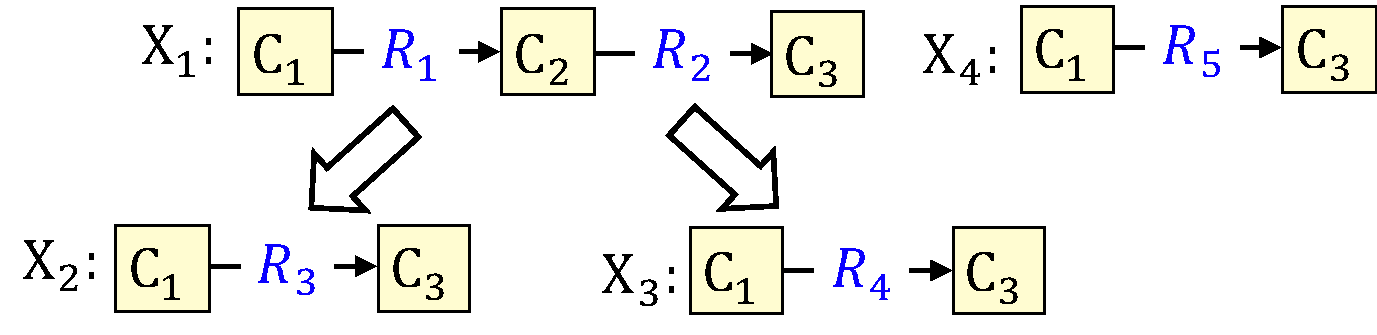
\includegraphics[width=7cm]{submissions/causal-meta-knowledge/figures/simulationv4.pdf}
\caption{The causal graph of relation paths, based on which the simulated KGs are generated .}
\label{fig:simulation}
% \vspace{-2pt}
\end{figure}

\begin{table}[h]
\caption{The parameters of conditional distributions.}
%\vspace{5pt}
\label{tab:simulation_set}
\centering
\scalebox{1}{
\begin{tabular}{c|cccc}
\hline
Conditions & $X_2|X_1=1$ & $X_2|X_1=0$ & $X_3|X_1=1$ & $X_3|X_1=0$ \\
\hline
Parameters & $p$=0.9 & $p$=0.1 & $p$=0.9 & $p$=0.1 \\
\hline
\end{tabular}}
% \vspace{-2pt}
\end{table}
% We generate simulated KGs based on a toy causal model specified in Fig.~\ref{fig:toy_example}, which includes five concepts and ten relations.
% More specifically, given $N$ entities for each concept, the facts containing the relations in the root nodes ($M_1$, $M_2$, $M_7$) of the causal graph are generated via Bernoulli distributions, whose probability mass function is $f(x)=p_r^x(1-p_r)^{1-x}$.
% For example, the entity pair $(e_1,e_3)$, where $e_1 \in \mathcal{E}_{C_1}$ and $e_3 \in \mathcal{E}_{C_3}$, the probability that the fact $<e_1,R_1,e_3> \in \mathcal{G}$ is $p_r$.
% % It means for any entity pair $(e_h,e_t)$, where $e_h \in \mathcal{E}_{C_h},\mathcal{E}_{C_t}$ and $R_i(C_h,C_t) \in \text{KG schema} \mathcal{S}$, the probability that the fact $R_i(e_h,e_t) \in \mathcal{T}$ is $p_r$.
% % we design the conditional  probabilistic distribution in SPRM based on which to sample the entity and facts in KG.
% And the facts in non-root nodes (e.g., $M_3$) are generated via the conditional probability distributions, which are Bernoulli distributions with parameter set $\mathbf{p}_{nr}$, given the facts information of parent node ($M_1$).
% For example, if there is a path instance of $M_1$ between $(e_1,e_3)$, then the probability of the existence of fact $<e_1,R_5,e_3>$ is $p_{M_1=1}$, otherwise is $p_{M_1=0}$.
% \yym{the value of all parameter of $p_nr$}

%


\noindent
{\bf Douban movie rating.}
Douban is a famous Chinese website for movie reviews, where users can rate and comment on any movie.
The rating range is from 1 to 5. A higher rating means that users like movies, while a lower rating means that users have negative feedback on movies.
We collect the real-world data from Douban\footnote{https://www.douban.com/} and construct a dataset (this dataset will be released), whose statistics are shown in Table~\ref{tab:dataset_statistics}.
Commonly, a movie with a score of 4 or 5 is identified as meeting the taste of users.
So we transform the original 5-level rating to a 2-level rating with a threshold of 4.
If the rating score is 4 or 5, the original relation \textit{Rate} is replaced by  \textit{HighRate}
We conduct the link prediction task on the relation \textit{HighRate}.
Because the raw data is too large and the relations between users and movies are very sparse, in this thesis, we first filter the 20 users who have made the most ratings and take the rating history of these users as the set of rating facts for our study.
The facts unrelated to the rating are also included in our experimental data.

\noindent
{\bf Hetionet}\cite{himmelstein2017systematic}
is a freely available knowledge database that integrates biomedical information from 29 prominent
bioinformatics resources.
Recently, Hetionet was successfully applied to drug repurposing tasks in terms of the link prediction task for relation \texttt{Treats}\cite{himmelstein2017systematic, ratajczak2022task}.

\textit{Why do we choose those two real datasets instead of other commonly used datasets, such as WN18, FB15k?}
In this paper, we focus on link prediction with the help of causal relationships between knowledge graph relations.
The core of causality lies in its asymmetry.
The commonly used KGs for link prediction algorithms contain many symmetrical relationships, e,g., \textit{hypernym} and \textit{hyponym} in WN18.
These symmetrical relationships may help with the link prediction task, but they go against the basic idea that causality is a one-way relationship.
We, therefore, chose datasets with specific application scenarios and rich causal semantics.

\subsubsection{\textbf{Metrics.}}
\textbf{For link prediction}, we employ the commonly used metrics mean reciprocal rank (MRR) and Hits@k~\cite{rossi2021knowledge,balazevic2019tucker,bordes2013translating}.
\begin{equation}
\label{eq:mrr}
\begin{aligned}
M R R=\frac{1}{|Q|} \sum_{q \in Q} \frac{1}{q}
\end{aligned}
\end{equation}

\begin{equation}
\label{eq:hitk}
\begin{aligned}
Hit@K=\frac{|\{q \in Q: q \leq K\}|}{|Q|}
\end{aligned}
\end{equation}
where $Q$ is the rank results, for each $q_i \in Q$ is the ranking of the desired results in the $i$-th query $(?,R_h,e_t)$.
In the case of ties in the calculation of $Q$, we use the mean rank to avoid misleading results\cite{rossi2021knowledge,ruffinelli2020you}.
% Common values for $K$ are 1, 3, 5, 10, we use $K=5$ in this paper.
Both MRR and His@k are the higher, the better.

\noindent
\textbf{The interpretability of causal rules} on the simulation dataset can be understood as the consistency between the mined causal rules and the actual causal structure.
Therefore, we evaluate baselines and our approach on the simulation dataset using precision, recall, and structural Hamming distance (SHD) as the evaluation metrics, which are commonly used evaluation metrics in causal structure discovery studies~\cite{zheng2018dags,zheng2020learning}.
% Since the performance of causal rule discovery is the foundation of our link prediction method.

\begin{equation}
\label{eq:precision}
\begin{aligned}
Precision=\frac{\# TFR}{\#FR};Recall=\frac{\# TFR}{\#ATR}
\end{aligned}
\end{equation}
Where $\#TFR$ is the number of right causal relationships discovered by an algorithm, $\#FR$ is the number of causal relationships discovered by an algorithm, and $\#ATR$ is the number of all causal relationships.
Both precision and recall are the higher, the better.
SHD calculates the difference between the learned graph and the ground truth graph by the number of edge insertions, deletions, or flips required to transform one graph into another.
The lower the SHD, the better.

\subsubsection{\textbf{Out-of-Distribution Link Prediction}}
Traditional machine learning methods are designed based on the assumption of independent and identically distributed (I.I.D) data.
This assumption means the training and test data come from the same distribution. However, the distribution of test data may alter due to changes in the test environment; such tasks are referred to as OoD tasks.
Traditional algorithms perform poorly on generalization problems due to the violation of I.I.D assumption.
Causality is seen as a stable inference mechanism in many research works on generalization problems.
So, in this work, we provide an out-of-distribution generalization task for the knowledge link prediction task for the first time.
On the one hand, the effect of causal metaknowledge on this task can be measured, and on the other, the performance of existing algorithms can be looked at.
We also evaluate the performance of the algorithms on I.I.D link prediction tasks.

In this paper, we design two OoD experimental scenarios.

\noindent
(1) \textit{Simulation dataset}:
We evaluate the link prediction performance under I.I.D and OoD settings, where the triples of root node $X_1$ are generated in testing under the same and different parameters with training.
In the training and I.I.D testing datasets, $p_{X_1}=0.5$.
In the OoD testing datasets, $p_{X_1} \in \{0.2,0.9\}$.
For $X_4$, $p_{X_4}$ maintains $0.9$ in training and testing.
The facts of the KGs are split into three parts:\textit{train}, \textit{test info}, and \textit{test}.
The facts in \textit{train} are used to learn the rule.
The effectiveness of the learned rule is assessed via the link prediction task on $R_3$.
The \textit{test info} part includes facts of new entities (did not appear in \textit{train}) on $R_1, R_2, R_4, R_5$, and \textit{test} part includes the queried facts on $R_3$.

\noindent
(2)\textit{Real datasets}:
It is impossible to explicitly change the data distribution since real data distribution is inaccessible for real datasets.
Recent research\cite{tang2020investigating,wu2021self} has suggested that graph models are biased towards nodes with larger degrees, which causes the bad performance of low-degree nodes in the test.
Therefore we construct the OoD datasets based on degree shift.
Specifically, given a query task $(?,R_h,e_t)$, we calculate the \textit{median} of degree\footnote{In this paper, we use the term "degree" to stand for the sum of in and out degrees} of known entities $e_t$ belonging to the triples $(e_h,R_h,e_t)$ in the training.
Then we bin the test queries by the degrees of the known entities $e_t$.
The degree range in each bucket is decided based on the sample size balance.
The test queries in the bucket, which the training median falls in, can be treated as the I.I.D test samples.
Others are the OoD samples.
The I.I.D bucket is labeled with $*$ in Table~\ref{tab:douban-mrr} and Table~\ref{tab:hetionet-mrr}.





\subsection{Performance of Link prediction task in Out-of-Distrition Settings}

\noindent
\textbf{Results on simulations.}
For the simulation dataset, we construct a OoD setting named as covariance shift, by changing the probability distribution of the root nodes in the test phase.
Table~\ref{tab:simulation_result} presents the methods in performance and demonstrates the effectiveness of the proposed \dname.
In particular, \dname~outperforms the baseline models under all metrics except the Hits@10 under I.I.D setting. This shows our method can give a stable and high-quality result, especially in the OOD setting.
Besides, compared with the baselines, the proposed \dname~ perform significantly better at the Hits@1 metric (at least 25\% absolute improvements that the second place under all settings), which suggests the our method are more suitable for scenarios with strict performance requirements, and this feature may achieved by the removal of association-based rules.

\begin{table}[h]
\caption{The results of link prediction on simulation datasets.}
\centering
\label{tab:simulation_result}
\scalebox{1.2}{
\begin{tabular}{c|c|l|cccc}
\hline
 \multirow{2}{*}{\textbf{Settings}}& \multirow{2}{*}{$\mathbf{p_{X_1}}$} & \multirow{2}{*}{\textbf{Method}} & \multirow{2}{*}{\textbf{MRR}} & \multicolumn{3}{c}{\textbf{Hits}} \\ \cline{5-7}
& & & &\textbf{@10} & \textbf{@3} & \textbf{@1} \\ \hline
\multirow{4}{*}{I.I.D} & \multirow{4}{*}{0.5}
& AMIE+ & 0.87 & \textbf{98.99} & 94.95 & 78.79\\
&  & AnyBURL & 0.87 &\textbf{98.99}&94.95 &78.79\\
&  & Neural-LP &  0.80 & \textbf{98.99} & 92.42& 66.16\\
& & RNNLogic & 0.87 & \textbf{98.99} & 94.95 & 78.79\\
&& \dname & \textbf{0.94} & 98.48&\textbf{97.98} &\textbf{90.91}\\

 \hline
\multirow{4}{*}{OOD} & \multirow{4}{*}{0.2}
& AMIE+ & 0.875 & 96.91 & 93.81 & 81.44 \\
&  & AnyBURL &  0.875 & 96.91&93.81 & 81.44\\
& & Neural-LP & 0.68 & 98.97 & 79.38 & 50.51\\
& & RNNLogic & 0.875 & 96.91 & 93.81 & 81.44 \\
&& \dname & \textbf{0.99} & \textbf{100}&\textbf{100} &\textbf{99.97}\\
 \hline
 \multirow{4}{*}{OOD} & \multirow{4}{*}{0.9}
& AMIE+ & 0.91 & \textbf{100} & 96.34 & 85.67 \\
&  & AnyBURL &  0.91 &\textbf{100} & 96.34 & 85.67\\
& & Neural-LP & 0.88 & \textbf{100} & 96.95 & 79.57\\
& & RNNLogic & 0.91 & \textbf{100} & 96.34 & 85.67 \\
&& \dname & \textbf{0.99} &  \textbf{100}& \textbf{99.70} & \textbf{99.09}\\
 \hline
\end{tabular}
}
\end{table}

% Also we considered the effect of different score functions on the link prediction performance.
% The results are shown in Tab.~\ref{tab:simulation_result}, and  can find that our method also works well for the simulated data, especially under OoD settings. Specifically, our model gets the best MRR and Hit@1 results, while AMIE+ and AnyBURL are the best methods for Hit@5 and Hit@10 for I.I.D setting. This may be because they tend to discover more rules, while our method aims to identity the causality more accurately, so fewer links are predicted.
% For OoD data, the proposed method surpasses all baseline models on all metrics, which fully support our motivation: building a link prediction algorithm with strong generalization ability.

% Overall, our method performs best for all three datasets. Also note although some baselines get the best results under some specific settings, they can not maintain a good performance for other settings or metrics. For example, TuckER gets the best MRR under 0-5 degree range, while performs worst with 30-60 degree range on Douban movie rating dataset. By contrast, the proposed CMLP can achieve best or competitive results for all settings.

% \yym{Prior systems for generating conjectures have either contributed genuinely useful research conjectures9 via methods that do not easily generalize to other mathematical areas10, or have dem- onstrated novel, general methods for finding conjectures11 that have not yet yielded mathematically valuable results.}


% \begin{table}[h]
% \caption{The results of link prediction on simulation datasets.}
% \centering
% \label{tab:simulation_result}
% \scalebox{1}{
% \begin{tabular}{c|c|l|cccc}
% \hline
%  \multirow{2}{*}{\textbf{Settings}}& \multirow{2}{*}{$\mathbf{p_{r}}$} & \multirow{2}{*}{\textbf{Method}} & \multirow{2}{*}{\textbf{MRR}} & \multicolumn{3}{c}{\textbf{Hits}} \\ \cline{5-7}
% & & & &\textbf{@1} & \textbf{@5} & \textbf{@10} \\ \hline
% \multirow{5}{*}{I.I.D} & \multirow{5}{*}{0.3}
% & AMIE+ & 0.734 & 0.589 & \textbf{0.948} & \textbf{1}\\
% &  & AnyBURL & 0.733 & 0.589 & \textbf{0.948} & \textbf{1}\\
% &  & Neural-LP &  0.58 & 0.41 & 0.743 & 0.769\\
% &  & RNNLogic &  0.603 & 0.461 & 0.666 & 0.666\\
% & & \dname & \textbf{0.785} & \textbf{0.692} & 0.897 & 0.897 \\

% %  \hline
% % \multirow{5}{*}{OOD} & \multirow{5}{*}{0.1}
% % & AMIE+ & 0.73 & 0.538 & \textbf{0.846} & \textbf{0.846} \\
% % &  & AnyBURL &  \textbf{0.782} & \textbf{0.615} & \textbf{0.846} & \textbf{0.846} \\
% % & & Neural-LP & 0.673 & 0.461 & 0.769 & 0.769\\
% % & & RNNLogic & 0.611 & 0.307 & 0.538 & 0.538\\
% % && \dname & 0.692 & 0.538 & 0.692 & 0.692\\
%  \hline
%  \multirow{5}{*}{OOD} & \multirow{5}{*}{0.8}
% & AMIE+ & 0.891 & 0.843 & \textbf{0.98} & \textbf{1} \\
% &  & AnyBURL &  0.893 & 0.843 & \textbf{0.98} & \textbf{1}\\
% & & Neural-LP & 0.885 & 0.843 & 0.941 & 0.98\\
% & & RNNLogic & 0.853 & 0.803 & 0.882 & 0.882\\
% && \dname & \textbf{0.909} &  \textbf{0.862} & \textbf{0.98} & \textbf{1}\\
%  \hline
% \end{tabular}
% }
% \end{table}
\noindent
\textbf{Results for Douban movie rating.}
Since we filtered the users of the Douban data, and the discrepancies of the degrees of experimental user nodes are close to each other.
Therefore, in this experiment, to construct the OoD scenario, we adopt the head prediction (? , HighRate, Movie), predicting the set of users who gave high ratings to movies.
Further, we bucketed the movie nodes in the test data according to their degree in the training data to observe the performance of the algorithm under different node prevalence.
The MRR and Hits@5 results shown in
Tab.~\ref{tab:douban-mrr} shows that the proposed CMLP get the best performance in the all OoD settings.
Especially, at least 25.8\% and 29.3 \% relative improvements that the second place on the MRR and Hits@5, respectively.
In the I.I.D setting, ~\dname~gets the second place on both MRR and Hits@5, lower than the representation-based method TuckER.
These results illustrate that for movie
rating datasets, the rules learned by our method can capture more general user preferences and give relatively accurate rating predictions for movies that are in different popularity.





% sum query head
\begin{table}[]
\centering
\caption{MRR (left) and Hits@5 (right) for Douban movie rating. The * marks columns that contain the I.I.D results. Other columns contain OoD results.}
\label{tab:douban-mrr}
\scalebox{1.2}{
\begin{tabular}{c|ccccc}
\hline
\multirow{2}{*}{\textbf{Methods}} & \multicolumn{4}{c}{\textbf{Degree Range}} \\ \cline{2-5}
          & \textbf{0-21*}   & \textbf{21-31}   & \textbf{31-39} & \textbf{39-60} \\ \hline
AMIE+     & 0.120 & 0.205 & 0.261 & 0.395 \\
AnyBURL   & 0.125 & 0.182  & 0.231 & 0.373 \\
Neural-LP & 0.078 & 0.097  & 0.126 & 0.217 \\
RNNLogic  & 0.072 & 0.086  & 0.097 & 0.161 \\
TuckER    & \textbf{0.287} & 0.186  &  0.186 & 0.149 \\
\dname      & 0.251 & \textbf{0.343}  & \textbf{0.392} & \textbf{0.497}\\ \hline
\end{tabular}
\quad
\begin{tabular}{c|ccccc}
\hline
\multirow{2}{*}{\textbf{Methods}} & \multicolumn{4}{c}{\textbf{Degree Range}} \\ \cline{2-5}
         & \textbf{0-21*}    & \textbf{21-31}   & \textbf{31-39} & \textbf{39-60}  \\ \hline
AMIE+        & 13.7 &30.7  & 39.4  & 68.3  \\
AnyBURL      & 15.1  & 26.0  & 33.2 & 64.6  \\
Neural-LP    & 0.1      & 0.6     & 3.4     & 60.0 \\
RNNLogic     & 1.6    & 4.7  & 7.2 & 13.5  \\
TuckER     & \textbf{50.3}   & 31.9   & 28.2  &  21.5 \\
\dname     & 40.9  & \textbf{60.0}  & \textbf{68.1} & \textbf{88.3}  \\ \hline
\end{tabular}}
\end{table}


% \begin{table}[]

% \caption{Hits@5 for Douban movie rating. The * marks columns that contain the I.I.D results. Other columns contain OoD results.}
% \label{tab:douban-hits1}
% \begin{tabular}{c|ccccc}
% \hline
% \multirow{2}{*}{\textbf{Methods}} & \multicolumn{4}{c}{\textbf{Degree Range}} \\ \cline{2-5}
%          & \textbf{0-21*}    & \textbf{21-31}   & \textbf{31-39} & \textbf{39-60}  \\ \hline
% AMIE+        & 13.7 &30.7  & 39.4  & 68.3  \\
% AnyBURL      & 15.1  & 26.0  & 33.2 & 64.6  \\
% Neural-LP    & 0.1      & 0.6     & 3.4     & 60.0 \\
% RNNLogic     & 1.6    & 4.7  & 7.2 & 13.5  \\
% TuckER     & \textbf{50.3}   & 31.9   & 28.2  &  21.5 \\
% \dname     & 40.9  & \textbf{60.0}  & \textbf{68.1} & \textbf{88.3}  \\ \hline
% \end{tabular}
% \end{table}

\noindent
\textbf{Results for drug repurposing on Hetionet.}
Consistent with the traditional setup of drug redirection, on Hetionet, we also use head predition (?, Treat, Disease), which is giving a Disease to predict new drugs. We also observe the performance of the algorithm under this task by bucketing for Disease node degrees.
Tab.~\ref{tab:hetionet-mrr} reports the MRR and Hits@5 on this dataset, and we can find that: our CMLP performs significantly better than other baselines on low-degree diseases (0-17), while AMIE+ and AnyBURL get better results on low-degree diseases (17-100).
These results indicate that our method can give more accurate drug discovery results for diseases with relatively low information.
And for diseases with richer information, the correlation-based inference rules give more accurate drug prediction.


\begin{table}[]
\centering
\caption{MRR(left) and Hits@5(right) for drug repurposing on Hetionet. The * marks columns that contain the I.I.D results. Other columns contain OoD results.}
\label{tab:hetionet-mrr}
\scalebox{1.2}{
\begin{tabular}{c|ccccc}
\hline
\multirow{2}{*}{\textbf{Methods}} & \multicolumn{4}{c}{\textbf{Degree Range}} \\ \cline{2-5}
    & \textbf{0-8*}    & \textbf{8-17}   & \textbf{17-31}  & \textbf{31-100} \\ \hline
AMIE+   & 0.103  & 0.085  & \textbf{0.132}  & 0.065 \\
AnyBURL  & 0.116   & 0.189  & 0.090  & \textbf{0.188} \\
Neural-LP & 0.027  & 0.014  & 0.009  & 0.009 \\
RNNLogic & 0.07  & 0.021  & 0.029  & 0.012 \\
TuckER  &  0.044  & 0.022    & 0.083   &  0.015 \\
\dname  & \textbf{0.248}  & \textbf{0.208}  & 0.095 & 0.093 \\ \hline
\end{tabular}
\quad
\begin{tabular}{c|cccc}
\hline
\multirow{2}{*}{\textbf{Methods}} & \multicolumn{4}{c}{\textbf{Degree Range}} \\ \cline{2-5}
  & \textbf{0-8*}    & \textbf{8-17}   & \textbf{17-31}  & \textbf{31-100} \\
  \hline
AMIE+      & 13.2  & 11.3  & \textbf{22.5} & 13.2  \\
AnyBURL     & 15.8  & \textbf{25.0}  & 9.6  & \textbf{23.7}   \\
Neural-LP   & 5.3      & 0     & 0      & 0      \\
RNNLogic  & 7.9  & 0  & 3.2      & 0      \\
TuckER    &  3.1   & 5.9  &  10.7  &  3.2   \\
\dname     & \textbf{26.31}  & \textbf{25.0} & 16.1 & 13.1  \\ \hline
\end{tabular}}
\end{table}

% \begin{table}[]

% \caption{MRR for drug repurposing on Hetionet. The * marks the range in which the mean of the training data falls.}
% \label{tab:hetionet-mrr}
% \begin{tabular}{c|ccccc}
% \hline
% \multirow{2}{*}{\textbf{Methods}} & \multicolumn{3}{c}{\textbf{Degree Range}} \\ \cline{2-4}
%     & \textbf{0-5}    & \textbf{5-15*}   & \textbf{15-30}   \\ \hline
% AMIE+   & 0.277  & 0.103  & 0.126   \\
% AnyBURL  & 0.28   & 0.177  & 0.134  \\
% Neural-LP & 0.036  & 0.016  & 0.011  \\
% RNNLogic & 0.149  & 0.038  & 0.023   \\
% TuckER  &  0.085  & 0.021    & 0.078    \\
% \dname  & \textbf{0.329}  & \textbf{0.327}  & \textbf{0.261} \\ \hline
% \end{tabular}
% \end{table}

% \begin{table}[]

% \caption{Hits@5 for drug repurposing on Hetionet. The * marks columns that contain the I.I.D results. Other columns contain OoD results.}
% \label{tab:hetionet-hits1}
% \begin{tabular}{c|cccc}
% \hline
% \multirow{2}{*}{\textbf{Methods}} & \multicolumn{4}{c}{\textbf{Degree Range}} \\ \cline{2-5}
%   & \textbf{0-8*}    & \textbf{8-17}   & \textbf{17-31}  & \textbf{31-100} \\
%   \hline
% AMIE+      & 13.2  & 11.3  & \textbf{22.5} & 13.2  \\
% AnyBURL     & 15.8  & \textbf{25.0}  & 9.6  & \textbf{23.7}   \\
% Neural-LP   & 5.3      & 0     & 0      & 0      \\
% RNNLogic  & 7.9  & 0  & 3.2      & 0      \\
% TuckER    &  3.1   & 5.9  &  10.7  &  3.2   \\
% \dname     & \textbf{26.31}  & \textbf{25.0} & 16.1 & 13.1  \\ \hline
% \end{tabular}
% \end{table}

% \begin{table}[]

% \caption{Hits@1 for drug repurposing on Hetionet. The * marks the range in which the mean of the training data falls.}
% \label{tab:hetionet-hits1}
% \begin{tabular}{c|cccc}
% \hline
% \multirow{2}{*}{\textbf{Methods}} & \multicolumn{3}{c}{\textbf{Degree Range}} \\ \cline{2-4}
%   & \textbf{0-5}    & \textbf{5-15*}  & \textbf{15-30}   \\ \hline
% AMIE+      & 0.111  & 0.02  & 0.027   \\
% AnyBURL     & 0.111  & 0.06  & 0.027     \\
% Neural-LP   & 0      & 0     & 0            \\
% RNNLogic  & 0.055  & 0.02  & 0          \\
% TuckER    &  0.071   & 0  &  0.064    \\
% \dname     & \textbf{0.166}  & \textbf{0.14}  & \textbf{0.138}   \\ \hline
% \end{tabular}
% \end{table}

\noindent


% \begin{table}[h]
% \caption{The results of link prediction on simulation datasets. The adopted score function is AVG.}
% \centering
% \label{tab:simulation_result2}
% \scalebox{1}{
% \begin{tabular}{c|c|l|cccc}
% \hline
%  \multirow{2}{*}{\textbf{Settings}}& \multirow{2}{*}{$\mathbf{p_{r}}$} & \multirow{2}{*}{\textbf{Method}} & \multirow{2}{*}{\textbf{MRR}} & \multicolumn{3}{c}{\textbf{Hits}} \\ \cline{5-7}
% & & & &\textbf{@1} & \textbf{@5} & \textbf{@10} \\ \hline
% \multirow{5}{*}{I.I.D} & \multirow{5}{*}{0.3}
% & AMIE+ & 0.829 & 0.717 & \textbf{0.974} & \textbf{1}\\
% &  & AnyBURL & 0.829 & 0.717 & \textbf{0.974} & \textbf{1}\\
% &  & Neural-LP &  0.619 & 0.435 & 0.769 & 0.769\\
% &  & RNNLogic &  0.684 & 0.589 & 0.666 & 0.666\\
% & & \dname & \textbf{0.868} & \textbf{0.82} & 0.897 & 0.897 \\

% %  \hline
% % \multirow{5}{*}{OOD} & \multirow{5}{*}{0.1}
% % & AMIE+ & \textbf{0.807} & \textbf{0.692} & \textbf{0.846} & \textbf{0.846} \\
% % &  & AnyBURL &  \textbf{0.807} & \textbf{0.692} & \textbf{0.846} & \textbf{0.846} \\
% % & & Neural-LP & 0.711 & 0.538 & 0.769 & 0.769\\
% % & & RNNLogic & 0.807 & 0.461 & 0.538 & 0.538\\
% % && \dname & 0.769 & \textbf{0.692} & 0.692 & 0.692\\
%  \hline
%  \multirow{5}{*}{OOD} & \multirow{5}{*}{0.8}
% & AMIE+ & 0.887 & 0.823 & \textbf{1} & \textbf{1} \\
% &  & AnyBURL &  0.887 & 0.823 & \textbf{1} & \textbf{1}\\
% & & Neural-LP & 0.85 & 0.784 & 0.98 & 0.98\\
% & & RNNLogic & 0.898 & 0.882 & 0.882 & 0.882\\
% && \dname & \textbf{1} &  \textbf{1} & \textbf{1} & \textbf{1}\\
%  \hline
% \end{tabular}
% }
% \end{table}

\subsection{Quality and Interpretability  of Causal Rules.}

As stated in Sec.~\ref{section:introduction}, the mined rules play a key role in our algorithm, and an important advantage of these rules is that they are well interpretable.
In this section, we will evaluate the quality and interpretability of rules mined by \dname~.


% % In this section, we explore the performance of~\dname~on causal rule mining.
% With the aid of simulation data, we can quantitatively evaluate the ability of different rule-based algorithms for the discovery of causal graph structure in Fig.~\ref{fig:toy_example}.
% In particular we introduce a classical algorithm PC\cite{abellan2006some}for causal discovery of propositional data as an additional baseline.
% The results are shown in Fig.\ref{fig:sim-graph}, and we can get the following observations:
% (i) The proposed show a good overall performs on all metrics, {\it i.e.} precision, recall, and SHD.
% (ii) The deep learning-based approaches, {\it i.e.} Neural-LP and RNNLogic, are hard to obtain good performances on these metrics. The low recall of them suggests that they have difficulty in mining interpretable rules.



% \begin{table*}[h]
% \caption{All rules whose head are $R_5$, $R_6$ and $R_9$, obtained by each algorithm learned on simulated dataset. The rules with red text are the wrong results which are not consistent with the generation process.\lsx{Why so few for CMLP}
% % The orange text denotes the weight of each rule with the form max-normalization(original weight)
% }.
% \label{tab:simulation_rule}
% \centering
% \scalebox{0.8}{
% \begin{tabular}{c|l|l|l}

% \hline
% \textbf{Method} & \textbf{Rules of $R_5$} & \textbf{Rules of $R_6$} & \textbf{Rules of $R_9$} \\

% \hline
% \multirow{3}{*}{\dname} &
% $R_5(C_1,C_2) \gets R_1(C_1,C_3), R_2(C_3,C_2)$ &
% $R_6(C_1,C_2) \gets R_3(C_1,C_4), R_4(C_4,C_2)$  &
% $R_9(C_1,C_2) \gets R_6(C_1,C_2)$ \\
% & & \color{red}{$R_6(C_1,C_2) \gets R_9(C_1,C_2)$} &
% $R_9(C_1,C_2) \gets R_7(C_1,C_5), R_8(C_5,C_2)$ \\
% & & $R_6(C_1,C_2) \gets R_1(C_1,C_3), R_2(C_3,C_2)$ &  \\
% \hline
% \multirow{6}{*}{AMIE+} &
% $R_5(C_1,C_2) \gets R_1(C_1,C_3), R_2(C_3,C_2)$ &
% $R_6(C_1,C_2) \gets R_3(C_1,C_4), R_4(C_4,C_2)$ &
% $R_9(C_1,C_2) \gets R_7(C_1,C_5), R_8(C_5,C_2)$ \\
% & \color{red}{$R_5(C_1,C_2) \gets R_6(C_1,C_2)$} &
% \color{red}{$R_6(C_1,C_2) \gets R_9(C_1,C_2)$} &
% $R_9(C_1,C_2) \gets R_6(C_1,C_2)$ \\
% & \color{red}{$R_5(C_1,C_2) \gets R_9(C_1,C_2)$} &
% $R_6(C_1,C_2) \gets R_1(C_1,C_3), R_2(C_3,C_2)$ &
% \color{red}{$R_9(C_1,C_2) \gets R_3(C_1,C_4), R_4(C_4,C_2)$} \\
% & \color{red}{$R_5(C_1,C_2) \gets R_7(C_1,C_5), R_8(C_5,C_2)$}
% & \color{red}{$R_6(C_1,C_2) \gets R_5(C_1,C_2)$} &
% \color{red}{$R_9(C_1,C_2) \gets R_{10}(C_1,C_2)$} \\
% & \color{red}{$R_5(C_1,C_2) \gets R_3(C_1,C_4), R_4(C_4,C_2)$} &
% \color{red}{$R_6(C_1,C_2) \gets R_{10}(C_1,C_2)$} &
% \color{red}{$R_9(C_1,C_2) \gets R_1(C_1,C_3), R_2(C_3,C_2)$} \\
% & \color{red}{$R_5(C_1,C_2) \gets R_{10}(C_1,C_2)$} &
% \color{red}{$R_6(C_1,C_2) \gets R_7(C_1,C_5), R_8(C_5,C_2)$} &
% \color{red}{$R_9(C_1,C_2) \gets R_5(C_1,C_2)$} \\

% \hline
% % $R_3(C_1,C_3) \gets R_1(C_1,C_2), R_2(C_2,C_3)$
% \multirow{6}{*}{AnyBURL} &
% $R_5(C_1,C_2) \gets R_1(C_1,C_3), R_2(C_3,C_2)$ &
% $R_6(C_1,C_2) \gets R_3(C_1,C_4), R_4(C_4,C_2)$ &
% $R_9(C_1,C_2) \gets R_7(C_1,C_5), R_8(C_5,C_2)$ \\ &
% $ \color{red}{R_5(C_1,C_2) \gets R_7(C_1,C_5), R_8(C_5,C_2)}$ &
% $ \color{red}{R_6(C_1,C_2) \gets R_9(C_1,C_2)}$ &
% $ R_9(C_1,C_2) \gets R_6(C_1,C_2)$ \\ &
% $ \color{red}{R_5(C_1,C_2) \gets R_{10}(C_1,C_2)}$ &
% $R_6(C_1,C_2) \gets R_1(C_1,C_3), R_2(C_3,C_2)$ &
% $ \color{red}{R_9(C_1,C_2) \gets R_{10}(C_1,C_2)}$ \\ &
% $ \color{red}{R_5(C_1,C_2) \gets R_6(C_1,C_2)}$ &
% $ \color{red}{R_6(C_1,C_2) \gets R_5(C_1,C_2)}$ &
% $ \color{red}{R_9(C_1,C_2) \gets R_3(C_1,C_4), R_4(C_4,C_2)}$ \\ &
% $ \color{red}{R_5(C_1,C_2) \gets R_9(C_1,C_2)}$ &
% $ \color{red}{R_6(C_1,C_2) \gets R_{10}(C_1,C_2)}$ &
% $ \color{red}{R_9(C_1,C_2) \gets R_1(C_1,C_3), R_2(C_3,C_2)}$ \\ &
% $ \color{red}{R_5(C_1,C_2) \gets R_3(C_1,C_4), R_4(C_4,C_2)}$ &
% $ \color{red}{R_6(C_1,C_2) \gets R_7(C_1,C_5), R_8(C_5,C_2)}$ &
% $ \color{red}{R_9(C_1,C_2) \gets R_5(C_1,C_2)}$ \\
% \hline

% \multirow{4}{*}{Neural-LP} &
% $ \color{red}{R_5(C_1,C_2) \gets R_6(C_1,C_2)}$ &
% $ \color{red}{R_6(C_1,C_2) \gets R_9(C_1,C_2)}$ &
% $ \color{red}{R_9(C_1,C_2) \gets R_{10}(C_1,C_2)}$ \\ &
% $ \color{red}{R_5(C_1,C_2) \gets R_9(C_1,C_2)}$ &
% $ \color{red}{R_6(C_1,C_2) \gets R_{10}(C_1,C_2)}$ &
% $ \color{red}{R_9(C_1,C_2) \gets R_5(C_1,C_2)}$ \\ &
% $ \color{red}{R_5(C_1,C_2) \gets R_{10}(C_1,C_2)}$ &
% $ \color{red}{R_6(C_1,C_2) \gets R_5(C_1,C_2)}$ &
% $R_9(C_1,C_2) \gets R_6(C_1,C_4)$ \\ &&&
% $ \color{red}{R_9(C_1,C_2) \gets R_9(C_1,C_2)}$ \\
% \hline

% \multirow{2}{*}{RNNLogic} &
% $ \color{red}{R_5(C_1,C_2) \gets R_6(C_1,C_2)}$ &
% $ \color{red}{R_6(C_1,C_2) \gets R_5(C_1,C_2)}$ &
% $R_9(C_1,C_2) \gets R_6(C_1,C_2)$ \\ &&
% $ \color{red}{R_6(C_1,C_2) \gets R_9(C_1,C_2)}$ &
% $ \color{red}{R_9(C_1,C_2) \gets R_{10}(C_1,C_2)}$ \\
% \hline
% % \tabucline[1pt]{-}
% \end{tabular}}
% \end{table*}


% \begin{figure*}[t]
%     \centering
%     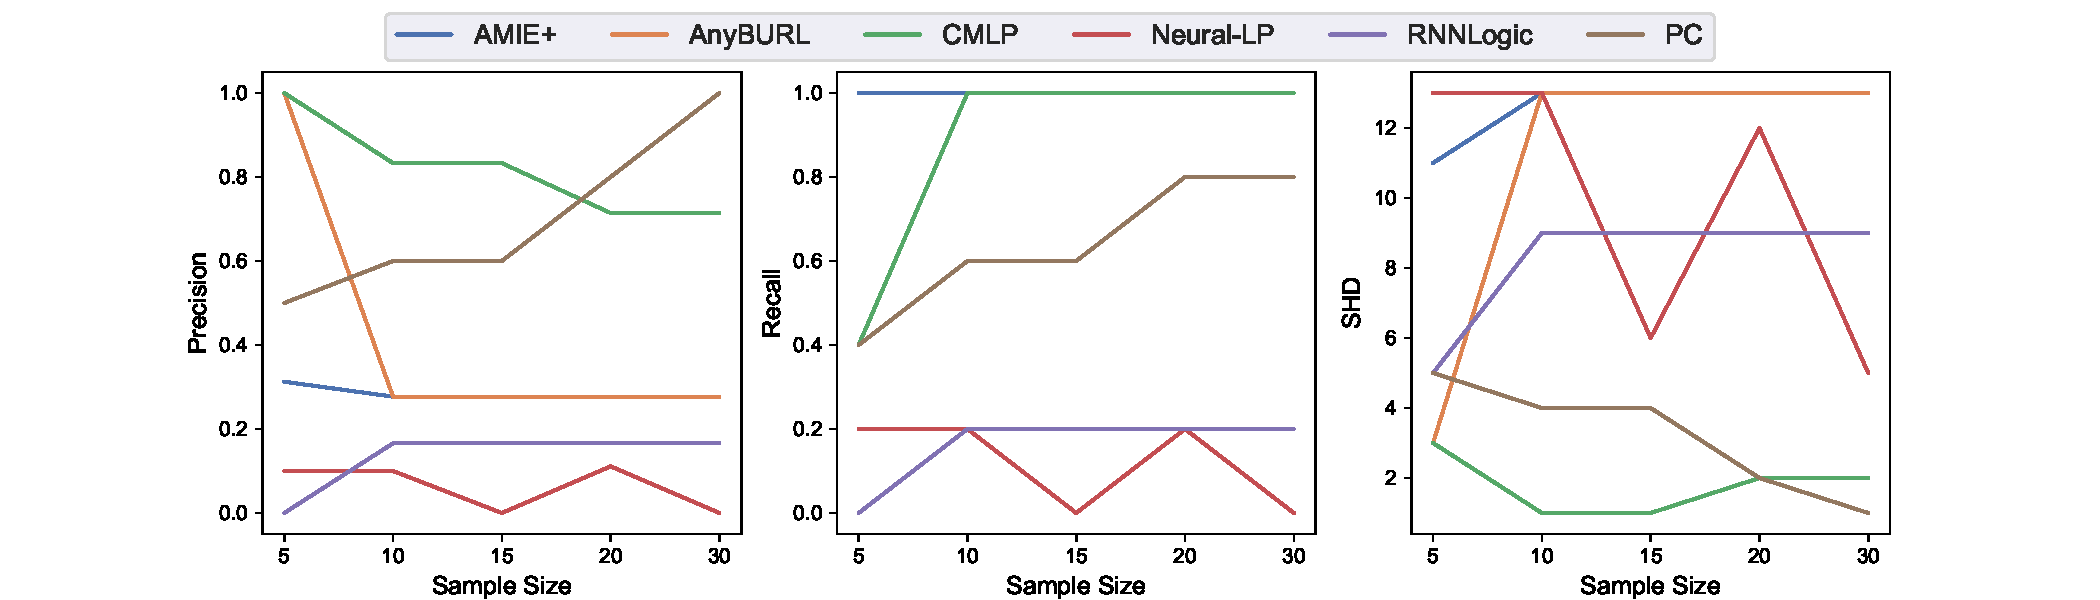
\includegraphics[trim=3cm 0cm 3cm 0cm, width=\linewidth, height=5cm]{figures/allin.pdf}
%     \caption{Precision, recall and SHD results on simulation datasets with differnet sample size. }
%     \label{fig:sim-graph}
% \end{figure*}
\noindent
\textbf{Quality of causal rules from simulations.}
The ground-truth causal graph of KGSs shown in Fig~\ref{fig:simulation}, and
Table~\ref{tab:simulation_rule_quality} shows the accuracy of estimated rules of different methods.
In particular, \dname~ accurately discovers two causal rules in Fig~\ref{fig:simulation} without any redundant rules.
In contrast, correlation-based methods report some non-causal rules.


\begin{table}[t]
\caption{Experimental results on simulation data with $p_{X_1}=0.5$, based on the metrics (precision, recall and SHD), which are commonly used to evaluate the estimated causal graph.}
%\vspace{5pt}
\label{tab:simulation_rule_quality}
\centering
\scalebox{1.2}{
\begin{tabular}{c|c|c|c}
\hline
\textbf{Method} & \textbf{Precision} $\uparrow$ & \textbf{Recall} $\uparrow$ & \textbf{SHD} $\downarrow$ \\
\hline
Neural-LP & 0 & 0& 10 \\
AMIE+ & 0.22 & \textbf{1.0}& 7 \\
RNNLogic & 0.22 & \textbf{1.0}& 7 \\
AnyBURL & 0.25 & \textbf{1.0}& 6 \\
\dname & \textbf{1.0} & \textbf{1.0} & \textbf{0} \\
\hline
\end{tabular}}
\vspace{-4pt}
\end{table}

\begin{table*}[h]
\caption{All rules whose head are $R_3$ and $R_5$, obtained by each algorithm learned on simulated dataset. The strikethroughs indicate the wrong results (there is no entities satisfying the rule).
The rules consistent with the generation process are in bold.
The orange text denotes the weight of each rule with the form max-normalization(original weight)}.

\label{tab:simulation_rule}
\centering
{\tiny
\scalebox{0.75}{
\begin{tabu}{c|l|l|l}
\tabucline[1pt]{-}
\textbf{Method} & \textbf{Rules of $R_3$ with $\mathbf{p_{X_1}=0.5}$} & \textbf{Rules of $R_3$ with $\mathbf{p_{X_1}=0.9}$} & \textbf{Rules of $R_5$}\\
\tabucline[1pt]{-}

\multirow{3}{*}{AMIE+} & \textcolor{orange}{1.00 (0.908)}   $\mathbf{R_3(C_1,C_3) \gets R_1(C_1,C_2), R_2(C_2,C_3)}$  & \textcolor{orange}{1.00 (0.900)}   $\mathbf{R_3(C_1,C_3) \gets R_1(C_1,C_2), R_2(C_2,C_3)}$ & \textcolor{orange}{1.00 (0.898)}   $R_5(C_1,C_3) \gets R_1(C_1,C_2), R_2(C_2,C_3)$\\

& \textcolor{orange}{0.91 (0.829)}   $R_3(C_1,C_3) \gets R_4(C_1,C_3)$ & \textcolor{orange}{0.99 (0.890)}   $R_3(C_1,C_3) \gets R_4(C_1,C_3)$ & \textcolor{orange}{0.99 (0.895)}   $R_5(C_1,C_3) \gets R_3(C_1,C_3)$ \\
&  \textcolor{orange}{0.55 (0.500)}   $R_3(C_1,C_3) \gets R_5(C_1,C_3)$  & \textcolor{orange}{0.91 (0.820)}   $R_3(C_1,C_3) \gets R_5(C_1,C_3)$ & \textcolor{orange}{0.99 (0.894)}   $R_5(C_1,C_3) \gets R_4(C_1,C_3)$\\
\hline
\multirow{3}{*}{AnyBURL}& \textcolor{orange}{1.00 (0.896)} $\mathbf{R_3(C_1,C_3) \gets R_1(C_1,C_2), R_2(C_2,C_3)}$ & \textcolor{orange}{1.00 (0.898)} $R_3(C_1,C_3) \gets R_4(C_1,C_3)$ & \textcolor{orange}{1.00 (0.907)} $R_5(C_1,C_3) \gets R_1(C_1,C_2), R_2(C_2,C_3)$\\
& \textcolor{orange}{0.92 (0.823)} $R_3(C_1,C_3) \gets R_4(C_1,C_3)$ &  \textcolor{orange}{0.99 (0.893)} $\mathbf{R_3(C_1,C_3) \gets R_1(C_1,C_2), R_2(C_2,C_3)}$ & \textcolor{orange}{0.99 (0.902)} $R_5(C_1,C_3) \gets R_3(C_1,C_3)$\\
& \textcolor{orange}{0.56 (0.501)} $R_3(C_1,C_3) \gets R_5(C_1,C_3)$ & \textcolor{orange}{0.91 (0.821)} $R_3(C_1,C_3) \gets R_5(C_1,C_3)$ & \textcolor{orange}{0.99 (0.897)} $R_5(C_1,C_3) \gets R_4(C_1,C_3)$ \\
\hline

\multirow{7}{*}{Neural-LP} & \textcolor{orange}{1.00 (0.318)}  \sout{$R_3(C_1,C_3) \gets R_4(C_1,C_2), R_4(C_2,C_3)$} & \textcolor{orange}{1.00 (0.757)}  \sout{$R_3(C_1,C_3) \gets R_1(C_1,C_2), R_1(C_2,C_3)$}  & \textcolor{orange}{1.00 (0.125)} \sout{$R_5(C_1,C_3) \gets R_4(C_1,C_2),R_3(C_2,C_3)$} \\
& \textcolor{orange}{0.99 (0.316)} \sout{$R_3(C_1,C_3) \gets R_4(C_1,C_2), R_5(C_2,C_3)$} & \textcolor{orange}{0.17 (0.128)} \sout{$R_3(C_1,C_3) \gets R_1(C_1,C_3)$} & \textcolor{orange}{0.78 (0.097)} \sout{$R_5(C_1,C_3) \gets R_3(C_1,C_2),R_3(C_2,C_3)$} \\
& \textcolor{orange}{0.31 (0.100)} \sout{$R_3(C_1,C_3) \gets R_5(C_1,C_2), R_4(C_2,C_3)$} & \textcolor{orange}{0.04 (0.056)} \sout{$R_3(C_1,C_3) \gets R_5(C_2,C_3), R_1(C_1,C_2)$} &\\
& \textcolor{orange}{0.31 (0.099)} \sout{$R_3(C_1,C_3) \gets R_5(C_1,C_2), R_5(C_2,C_3)$} & \textcolor{orange}{0.05 (0.035)} \sout{$R_3(C_1,C_3) \gets R_4(C_2,C_1), R_1(C_3,C_2)$} &\\
& \textcolor{orange}{0.23 (0.073)} $R_3(C_1,C_3) \gets R_4(C_1,C_3)$ & \textcolor{orange}{0.03 (0.025)} $\mathbf{R_3(C_1,C_3) \gets R_1(C_1,C_2), R_2(C_2,C_3)}$\\
& \textcolor{orange}{0.09 (0.028)} \sout{$R_3(C_1,C_3) \gets R_4(C_1,C_2), R_4(C_2,C_3)$} & \\
& \textcolor{orange}{0.07 (0.023)} $R_3(C_1,C_3) \gets R_5(C_1,C_3)$ &\\
\hline

\multirow{3}{*}{RNNLogic} & \textcolor{orange}{1.00 (0.076)}   $\mathbf{R_3(C_1,C_3) \gets R_1(C_1,C_2), R_2(C_2,C_3)}$  & \textcolor{orange}{1.00 (0.071
)}   $\mathbf{R_3(C_1,C_3) \gets R_1(C_1,C_2), R_2(C_2,C_3)}$ & \textcolor{orange}{1.00 (0.220)}   $R_5(C_1,C_3) \gets R_3(C_1,C_3)$\\

& \textcolor{orange}{0.58 (0.044)}   $R_3(C_1,C_3) \gets R_4(C_1,C_3)$ & \textcolor{orange}{0.49 (0.035)}   $R_3(C_1,C_3) \gets R_4(C_1,C_3)$ & \textcolor{orange}{0.28 (0.060)}   $R_5(C_1,C_3) \gets R_4(C_1,C_3)$ \\
&  \textcolor{orange}{0.13 (0.010)}   $R_3(C_1,C_3) \gets R_5(C_1,C_3)$  & \textcolor{orange}{0.14 (0.010)}   $R_3(C_1,C_3) \gets R_5(C_1,C_3)$ & \textcolor{orange}{0.20 (0.045)}   $R_5(C_1,C_3) \gets R_1(C_1,C_2), R_2(C_2,C_3)$\\
\hline


{\dname} & \textcolor{orange}{1.00 (122.797)} $\mathbf{R_3(C_1,C_3) \gets R_1(C_1,C_2), R_2(C_2,C_3)}$ & \textcolor{orange}{1.00 (20.061)} $\mathbf{R_3(C_1,C_3) \gets R_1(C_1,C_2), R_2(C_2,C_3)}$ & -\\

\tabucline[1pt]{-}
\end{tabu}}
}
\end{table*}

\noindent
\textbf{Interpretability of causal rules}
% For rules from the simulation, we analyze all methods' results, whose heads are $R_5$ and $R_6$, and $R_9$ and the results are shown in Table~\ref{tab:simulation_rule} .
% % The rules follow the causal mechanism are in bold.
% There is only one causal rule for $R_5$, which is $R_5(C_1,C_2) \gets R_1(C_1,C_3), R_2(C_3,C_2)$.
% AMIE+, AnyBURL, and \dname~find this causal rule.
% Besides this causal rule, the results of AMIE+ and AnyBURL also include other rules, such as $R_5(C_1,C_2) \gets R_6(C_1,C_2)$ and $R_5(C_1,C_2) \gets R_9(C_1,C_3)$.
% % Especially, for AMIE+ and AnyBURL, note that the weights of $R_3(C_1,C_3) \gets R_4(C_1,C_3)$ are very close to the weights of $R_3(C_1,C_3) \gets R_1(C_1,C_2)$, $ R_2(C_2,C_3)$.
% % It means the algorithms think these two rules have the similar interpretability for the head relation $R_3$.
% % With the change of root node $X_1$'s distribution(from $p_{X_1}=0.5$ to $p_{X_1}=0.9$), AnyBURL even report the higher weight for the rule $R_3(C_1,C_3) \gets R_5(C_1,C_3)$.
% % According to the generation mechanism, the existence of $R_3$ between entities $e_i$ and $e_j$ is independent with whether there is $R_4$ and $R_5$ between $e_i$ and $e_j$.
% % AMIE+ and AnyBURL still return these association rules with high weights, because they only consider whether $R_3$ and $R_4$ co-occur frequently, but not the reason of the co-occurrence.
% The end-to-end deep-model based method(Neural-LP and RNNLogic) fail to discover any correct rules for $R_5$.
Moreover, for the simulation dataset, we analyze all methods' results, whose heads are $R_3$ and $R_5$, and the results are shown in Table~\ref{tab:simulation_rule} (We omit results of $R_4$, since $R_3$ and $R_4$ are symmetric in the causal graph).
The rules follow the causal mechanism are in bold.
There is only one causal rule for $R_3$, which is $R_3(C_1,C_3) \gets R_1(C_1,C_2), R_2(C_2,C_3)$.
AMIE+, AnyBURL, RNNLogic and \dname~find this causal rule.
Besides this causal rule, the results of AMIE+, RNNLogic and AnyBURL also include other rules, such as $R_3(C_1,C_3) \gets R_4(C_1,C_3)$ and $R_3(C_1,C_3) \gets R_5(C_1,C_3)$.
Especially, for those three methods, note that the weights of $R_3(C_1,C_3) \gets R_4(C_1,C_3)$ are very close to the weights of $R_3(C_1,C_3) \gets R_1(C_1,C_2)$, $ R_2(C_2,C_3)$.
It means the algorithms think these two rules have the similar interpretability for the head relation $R_3$.
With the change of root node $X_1$'s distribution(from $p_{X_1}=0.5$ to $p_{X_1}=0.9$), AnyBURL even report the higher weight for the rule $R_3(C_1,C_3) \gets R_5(C_1,C_3)$.
According to the generation mechanism, the existence of $R_3$ between entities $e_i$ and $e_j$ is independent with whether there is $R_4$ and $R_5$ between $e_i$ and $e_j$.
AMIE+, AnyBURL and RNNLogic still return these association rules with high weights, because they only consider whether $R_3$ and $R_4$ co-occur frequently, but not the reason of the co-occurrence.
The end-to-end completion-oriented method, Neural-LP, also return some wrong results, such as the top 1 rule $R_3(C_1,C_3) \gets R_4(C_1,C_2), R_4(C_2,C_3)$, which can not be satisfied by any entities in KG.
The results in~\cite{sadeghian2019drum} show the same phenomenon.
The intermediate results of the completion-oriented method is incomprehensible sometimes.


Furthermore, We sort the rules generated by each algorithm based on their assigned weights and show the five top rules from Douban and Hetionet in Tab.~\ref{tab:rules_recom_result} and Tab.~\ref{tab:rule_hetionet}, respectively.
The results in Tab.~\ref{tab:rules_recom_result} suggests that the ratings for the target movie are highly related to other movies which share the same staff, such as writer, actors, director, etc.
According to the rating results, \dname~ finds a strong causal relationship between the rating of the movie and its editor than other pairs.
The top rules generated by AMIE+ and AnyBURL focus on other shared staffs, but the shared staff has different roles in the target movie and the movie in path.
Those rules of AMIE+ and AnyBURL are hard to be satisfied for most queries.
% By contrast, our mined rules suggest the ratings are determined by the subjective opinions of the users, while the mined rules from other algorithms, including AnyBURL, present the ratings are depended on others related events.
It is worth noting that RNNlogic report the `fan' rules  will impact the users' rating, but \dname~ excludes this kind of rules.
Our results suggest the working ability of the movie's stuff ({\it e.g.} actor or writer) should be the root cause of the users' rate, instead of the followers of the stuff.
From the rules from Hetionet, we can see
% Similar to the results on simulation dataset,
the learned rules are broadly divided into two classes, those in which the target drug and disease are connected by therapeutic information about the similar disease and drug, and those in which the target drug and disease are connected by commonly associated genes.
Further, we find that the rules mined by AnyBURL also contain rules for reasoning through shared side effects.



% Logically incorrect rules are highlighted by italic-red. This experiment shows two of the three top ranked rules generated by Neural LP are incorrect (for both head predicates wif e and son
\begin{table*}[t]
\centering
\caption{Top 5 Rules to infer HighRate(User, Movie) given by the methods. The strikethroughs indicate the wrong results (there is no entities satisfying the rule).
}
\label{tab:rules_recom_result}
\vspace{-1pt}
{\tiny
\begin{tabular}{c|l}
\hline
\textbf{Method} & \multicolumn{1}{c}{\textbf{ Top rules to infer HighRate(User, Movie)}} \\
\hline

\multirow{5}{*}{AMIE+} &
\textcolor{orange}{1.00 (0.565)} HighRate(User,Movie) $\gets$ HighRate(User,Movie1), Writer(Person,Movie1),Director(Person,Movie)\\
& \textcolor{orange}{0.98 (0.556)} HighRate(User,Movie) $\gets$ HighRate(User,Movie1), Director(Person,Movie1), Writer(Person,Movie)\\
& \textcolor{orange}{0.87 (0.489)} HighRate(User,Movie) $\gets$ HighRate(User,Movie1), Writer(Person,Movie1), Actress(Person,Movie)\\
& \textcolor{orange}{0.74 (0.417)} HighRate(User,Movie) $\gets$ HighRate(User,Movie1), Director(Person,Movie1), Actor(Person,Movie)\\
& \textcolor{orange}{0.72 (0.405)} HighRate(User,Movie) $\gets$ HighRate(User,Movie1), Actress(Person,Movie1), Writer(Person,Movie)\\
\hline

\multirow{5}{*}{AnyBURL} &
\textcolor{orange}{1.00 (0.400)} HighRate(User,Movie) $\gets$ HighRate(User,Movie1), Composer(Person,Movie1), Actor(Person,Movie)\\
& \textcolor{orange}{0.99(0.397)} HighRate(User,Movie) $\gets$ HighRate(User,Movie1), Producer(Person,Movie1), Director(Person,Movie)\\
& \textcolor{orange}{0.97 (0.386)} HighRate(User,Movie) $\gets$ HighRate(User,Movie1), Director(Person,Movie1), Actress(Person,Movie)\\
& \textcolor{orange}{0.89 (0.355)} HighRate(User,Movie) $\gets$ HighRate(User,Movie1), Writer(Person,Movie1), Actress(Person,Movie)\\
& \textcolor{orange}{0.85 (0.340)} HighRate(User,Movie) $\gets$ HighRate(User,Movie1), Editor(Person,Movie1), Editor(Person,Movie)\\
\hline



\multirow{2}{*}{Neural-LP}
& \textcolor{orange}{1.00 (0.120)} HighRate(User,Movie) $\gets$ HighRate(User,Movie1), HighRate(User1,Movie1), HighRate(User1,Movie)\\
& \textcolor{orange}{0.28 (0.034)} HighRate(User,Movie) $\gets$ HighRate(User,Movie1), MovieType(Movie1,Type), MovieType(Movie,Type)\\
\hline


\multirow{5}{*}{RNNLogic} &
\textcolor{orange}{1.00 (0.011)} HighRate(User,Movie) $\gets$ Fan(User,Person),Editor(Person,Movie)\\
&\textcolor{orange}{0.45 (0.005)} HighRate(User,Movie) $\gets$ Fan(User,Person),Actor(Person,Movie)\\
&\textcolor{orange}{0.36 (0.004)} HighRate(User,Movie) $\gets$ Fan(User,Person),Director(Person,Movie)\\
&\textcolor{orange}{0.36 (0.004)} HighRate(User,Movie) $\gets$ Fan(User,Person),Writer(Person,Movie)\\
&\textcolor{orange}{0.36 (0.004)} HighRate(User,Movie) $\gets$ Fan(User,Person),Composer(Person,Movie)\\
\hline

\multirow{5}{*}{\dname} &
\textcolor{orange}{1.00 (0.034)} HighRate(User,Movie) $\gets$ HighRate(User,Movie1), Editor(Person,Movie1), Editor(Person,Movie)\\

& \textcolor{orange}{0.12 (0.004)} HighRate(User,Movie1) $\gets$ HighRate(User,Movie1),Cinematographer(Person,Movie),Cinematographer(Person,Movie)
\\
& \textcolor{orange}{0.06 (0.002)} HighRate(User,Movie1) $\gets$ HighRate(User,Movie1),Writer(Person,Movie),Writer(Person,Movie)\\
& \textcolor{orange}{0.06 (0.002)} HighRate(User,Movie1) $\gets$ HighRate(User,Movie1),Actress(Person,Movie),Actress(Person,Movie)\\
& \textcolor{orange}{0.03 (0.001)} HighRate(User,Movie1) $\gets$ HighRate(User,Movie1),Director(Person,Movie),Actor(Person,Movie)\\
\hline
\end{tabular}
}
\end{table*}


\begin{table*}
\centering
\caption{Top 5 Rules to infer Treats(Compound, Disease) given by the methods. For brevity, we use `C' and `D' for compound and disease, respectively.}
\label{tab:rule_hetionet}
{\tiny
\begin{tabular}{c|l}
    \hline
    \textbf{Method} & \multicolumn{1}{c}{\textbf{ Top rules to infer Treats(Compound, Disease)}} \\ \hline
    \multirow{5}{*}{AMIE+} &
\textcolor{orange}{1.00 (0.393)}
Treats(C, D) $\gets$ Resembles(C,C1), Treats(C1, D)
    \\
& \textcolor{orange}{0.82 (0.322)}
Treats(C, D) $\gets$ Resembles(C1,C),Treats(C1, D)
\\
& \textcolor{orange}{0.42 (0.167)} Treats(C, D) $\gets$ Downregulates(C,Gene1), Associates(D,Gene1)
\\
& \textcolor{orange}{0.38 (0.151)} Treats(C, D) $\gets$ Downregulates(C,Gene1), Upregulates(D,Gene1)
 \\
& \textcolor{orange}{0.37 (0.144)} Treats(C, D) $\gets$ Binds(C,Gene1), Upregulates(D,Gene1)
\\


\hline
\multirow{5}{*}{AnyBURL} & \textcolor{orange}{1.00 (0.319)}
Treats(C, D) $\gets$ Includes(PharmacologicClass1,C),Includes(PharmacologicClass1,C1),Treats(C1, D)
 \\
& \textcolor{orange}{0.60 (0.192)}
Treats(C, D) $\gets$ Resembles(C1,C),Treats(C1, D)
 \\
& \textcolor{orange}{0.52 (0.166)}
Treats(C, D) $\gets$ Resembles(C1,C),Resembles(C1,C2),Treats(C2, D)
 \\
& \textcolor{orange}{0.31 (0.098)}
Treats(C, D) $\gets$ Resembles(C1,C),Resembles(C2,C1),Treats(C2, D)
 \\
& \textcolor{orange}{0.24 (0.077)}
Treats(C, D) $\gets$ Treats(C, D1), Resembles(D1,D)
 \\ \hline


\multirow{1}{*}{Neural-LP} &
\textcolor{orange}{1.00 (0.659)}
Treats(C, D) $\gets$ Treats(C, D1), Treats(C1, D1),Treats(C1, D)
\\ \hline



\multirow{2}{*}{RNNLogic} &
\textcolor{orange}{1.00 (0.00007)}
Treats(C, D) $\gets$ Resembles(C, C1),Treats(C1, D)
 \\
& \textcolor{orange}{1.00 (0.00007)}

Treats(C, D) $\gets$ Resembles(C, C1),
Resembles(C1, C2),Treats(C2, D)
\\ \hline


\multirow{5}{*}{\dname} &
\textcolor{orange}{1.00 (269.00))}
Treats(C, D) $\gets$ Treats(C, D1),Resembles(D1, D2),Resembles(D, D2)
 \\
    & \textcolor{orange}{0.85 (229.32))}
Treats(C, D) $\gets$ Includes(PharmacologicClass1, C),Includes(PharmacologicClass1, C1),Treats(C1, D)

\\
    & \textcolor{orange}{0.83 (224.37))}
Treats(C, D) $\gets$
Treats(C, D1),Resembles(D2, D1),Resembles(D2, D)
\\
    & \textcolor{orange}{0.58 (155.18))}
Treats(C, D) $\gets$ Treats(C, D1),Treats(C1, D1),Treats(C1, D)


\\
    & \textcolor{orange}{0.10 (26.52))}
 Treats(C, D) $\gets$
 Treats(C, D1),
 Resembles(D2,D1),
 Resembles(D,D1)

    \\ \hline

\end{tabular}
}
\end{table*}


% \begin{table*}
% \caption{Top Rules to infer $User\stackrel{Rate}{\longrightarrow}Movie$ given by the methods.}
% \label{tab:rule_douban}
% \begin{tabular}{c|l}
%     \hline
%     \textbf{Method} & \multicolumn{1}{c}{\textbf{ Top rules to infer $User\stackrel{Rate}{\longrightarrow}Movie$}} \\ \hline
%     \multirow{3}{*}{AMIE+} &
%     1. $User\stackrel{Fan}{\longrightarrow}Person\stackrel{Director}{\longrightarrow}Movie$ \\
%     & 2. $User\stackrel{Fan}{\longrightarrow}Person\stackrel{Writer}{\longrightarrow}Movie$ \\
%     & 3. $User\stackrel{Rate}{\longrightarrow}Movie1\stackrel{Director}{\longleftarrow}Person\stackrel{Director}{\longrightarrow}Movie$ \\ \hline
%     \multirow{3}{*}{AnyBURL} &  1. $User\stackrel{Rate}{\longrightarrow}Movie1\stackrel{Wish}{\longleftarrow}User1\stackrel{Rate}{\longrightarrow}Movie$ \\
%     & 2. $User\stackrel{Rate}{\longrightarrow}Movie1\stackrel{Director}{\longleftarrow}Person\stackrel{Actor}{\longrightarrow}Movie$ \\
%     & 3. $User\stackrel{Rate}{\longrightarrow}Movie1\stackrel{Producer}{\longleftarrow}Person\stackrel{Actor}{\longrightarrow}Movie$ \\ \hline
%     \multirow{3}{*}{Neural-LP} & 1. $User\stackrel{Rate}{\longrightarrow}Movie1\stackrel{Rate}{\longleftarrow}User1\stackrel{Rate}{\longrightarrow}Movie$ \\
%     & 2. $User\stackrel{Rate}{\longrightarrow}Movie1\stackrel{titleType}{\longleftarrow}MovieType\stackrel{titleType}{\longrightarrow}Movie$ \\
%     & 3. $User\stackrel{Wish}{\longrightarrow}Movie1\stackrel{archivesound}{\longleftarrow}Person\stackrel{archivesound}{\longrightarrow}Movie$ \\ \hline
%     \multirow{3}{*}{RNNLogic} & 1. $User\stackrel{Fan}{\longrightarrow}Person\stackrel{Actor}{\longrightarrow}Movie$ \\
%     & 2. $User\stackrel{Fan}{\longrightarrow}Person\stackrel{Director}{\longrightarrow}Movie$ \\
%     & 3. $User\stackrel{Fan}{\longrightarrow}Person\stackrel{Writer}{\longrightarrow}Movie$ \\ \hline
%     \multirow{3}{*}{\dname} & 1. $User\stackrel{Rate}{\longrightarrow}Movie1\stackrel{Writer}{\longleftarrow}Person\stackrel{Writer}{\longrightarrow}Movie$ \\
%     & 2. $User\stackrel{Rate}{\longrightarrow}Movie1\stackrel{Actress}{\longleftarrow}Person\stackrel{Actress}{\longrightarrow}Movie$ \\
%     & 3.$User\stackrel{Rate}{\longrightarrow}Movie1\stackrel{Director}{\longleftarrow}Person\stackrel{Actor}{\longrightarrow}Movie$ \\ \hline
% \end{tabular}
% \end{table*}

% \begin{table*}[t]
% \centering
% \caption{Top 3 Rules of HighRate given by the methods.The strikethroughs indicate the wrong results (there is no entities satisfying the rule).
% The orange text denotes the weight of each rule with the form max-normalization(original weight)}
% \label{tab:rules_recom_result}
% \vspace{-1pt}
% \begin{tabular}{c|l}
% \hline
% \textbf{Method} & \multicolumn{1}{c}{\textbf{Rules of HighRate}} \\
% \hline
% \multirow{3}{*}{Neural-LP} &
% \textcolor{orange}{1.00 (0.636)} \sout{HighRate(User,Movie) $\gets$ Saw(User1,Movie), Saw(User2,User1)}\\
%  &    \textcolor{orange}{0.50 (0.320)} \sout{HighRate(User,Movie) $\gets$ Saw(User1,Movie), Saw(User2,User1),Saw(User,User2)} \\
%   &  \textcolor{orange}{0.02(0.011)}  HighRate(User,Movie) $\gets$ Saw(User, Movie)\\
% \hline
% \multirow{3}{*}{AMIE+} &
% \textcolor{orange}{1.00 (0.662)} HighRate(User,Movie) $\gets$ Fan(User, Person), Director(Person,Movie) \\
% & \textcolor{orange}{0.99 (0.658)} HighRate(User,Movie) $\gets$ Fan(User, Person), Writer(Person,Movie) \\
% & \textcolor{orange}{0.85 (0.565)} HighRate(User,Movie) $\gets$ HighRate(User,Movie1), Writer(Person,Movie1),Director(Person,Movie)\\
% \hline
% \multirow{5}{*}{AnyBURL} &
% \textcolor{orange}{1.00 (0.286)} HighRate(User,Movie) $\gets$ HighRate(User,Movie1), Wish(User1,Movie1),HighRate(User1,Movie) \\
% & \textcolor{orange}{0.97 (0.276)} HighRate(User,Movie) $\gets$ HighRate(User,Movie1), Director(Person,Movie1),Actor(Person,Movie)
% \\
% & \textcolor{orange}{0.97 (0.276)} HighRate(User,Movie) $\gets$ HighRate(User,Movie1), Producer(Person,Movie1),Actor(Person,Movie)\\
% & $\dots$ \\
% & \textcolor{orange}{0.983 (0.236)} HighRate(User,Movie) $\gets$ Fan(User,Person), Director(Person,Movie) \\
% \hline
% \multirow{3}{*}{RNNLogic} &
% \textcolor{orange}{1.00 (0.0048)} HighRate(User,Movie) $\gets$ Fan(User,Person), Actor(Person,Movie) \\
% & \textcolor{orange}{0.875 (0.0042)} HighRate(User,Movie) $\gets$ Fan(User,Person), Director(Person,Movie) \\
% & \textcolor{orange}{0.85 (0.0041)} HighRate(User,Movie) $\gets$ Fan(User,Person), Writer(Person,Movie) \\

% \hline
% \multirow{3}{*}{\dname} &
% \textcolor{orange}{1.00 (0.035)} HighRate(User,Movie) $\gets$ HighRate(User,Movie1),Writer(Person,Movie1),Writer(Person,Movie) \\
% & \textcolor{orange}{0.06 (0.002)} HighRate(User,Movie1) $\gets$ HighRate(User,Movie1),Actress(Person,Movie),Actress(Person,Movie)
% \\
% & \textcolor{orange}{0.06 (0.002)} HighRate(User,Movie1) $\gets$ HighRate(User,Movie1),Director(Person,Movie),Actor(Person,Movie)\\
% \hline
% \end{tabular}
% \end{table*}

% We conducted an experimental study in which we investigated the performance of the learned causal rules in two aspects: the explainability to the KG and the usefulness for downstream task, such as link prediction.
% Our main goal is to provide insight into
% \begin{itemize}
%     \item the explainability of the learned causal rules to the KG.
%     \item the effectiveness of the learned causal rules or downstream task, such as link prediction.
%     \item the empirical conclusions for the hyper-parameters and alternative algorithms in our framework.
% \end{itemize}
% Furthermore, we briefly summarize the experiment designs to achieve the above-mentioned the goal under the available resources.

% Goal 1 	$\Rightarrow$ We use the simulation KG to quantitatively evaluate the learned causal rules from KG, since the causal relationships are inaccessible for real dataset\footnote{This is the most commonly used way for the evaluation of the causal discovery methods in both relational and propositional data\cite{zheng2018dags, lee2016learning}}.
% Meanwhile, the case study for real data will be introduced to qualitatively discuss the quality of mined rules.

% Goal 2 	$\Rightarrow$ 